% RG-TTA: Regime-Guided Meta-Control for Test-Time Adaptation in Streaming Time Series
% IEEE TNNLS submission version (10-12 pages)
\documentclass[journal]{IEEEtran}

% --- Core packages ---
\usepackage[utf8]{inputenc}
\usepackage[T1]{fontenc}
\usepackage{amsmath,amssymb,amsthm}
\usepackage{graphicx}
\usepackage{booktabs}
\usepackage[hyphens]{url}
\usepackage[breaklinks=true,hidelinks,hypertexnames=false]{hyperref}
\usepackage{cite}
\usepackage{xcolor}
\usepackage{multirow}
\usepackage{enumitem}
\usepackage{algorithm}
\usepackage{algorithmic}
\usepackage[section]{placeins}
\usepackage{stfloats}
\usepackage{microtype}

% --- Widow/orphan control ---
\widowpenalty=10000
\clubpenalty=10000
\displaywidowpenalty=10000

% --- Float placement tuning ---
\renewcommand{\topfraction}{0.9}
\renewcommand{\bottomfraction}{0.9}
\renewcommand{\textfraction}{0.1}
\renewcommand{\floatpagefraction}{0.8}
\renewcommand{\dbltopfraction}{0.9}
\renewcommand{\dblfloatpagefraction}{0.8}
\setcounter{topnumber}{4}
\setcounter{bottomnumber}{4}
\setcounter{totalnumber}{8}
\setcounter{dbltopnumber}{4}

% --- Theorem environments ---
\newtheorem{proposition}{Proposition}
\newtheorem{theorem}{Theorem}
\newtheorem{corollary}{Corollary}
\newtheorem{definition}{Definition}

% --- IEEEtran proof environment fix ---
\renewenvironment{proof}[1][Proof]{\noindent\textit{#1.}\space}{\hfill$\blacksquare$\par\medskip}

% Repository
\newcommand{\repourl}{\url{https://github.com/IndarKarhana/RGTTA-Regime-Guided-Test-Time-Adaptation}}

\begin{document}

\title{RG-TTA: Regime-Guided Meta-Control for Test-Time Adaptation in Streaming Time Series}

\author{Indar~Kumar,
Akanksha~Tiwari,
Sai~Krishna~Jasti,
and~Ankit~Hemant~Lade%
\thanks{Code and data are available at \repourl.}%
\thanks{I.~Kumar, A.~Tiwari, S.~K.~Jasti, and A.~H.~Lade are independent researchers
(e-mail: indarkarhana@gmail.com, akankshat2803@gmail.com,
jsaikrishna379@gmail.com, ankitlade12@gmail.com).}}

\maketitle

% ============================================================
\begin{abstract}
% ============================================================

Test-time adaptation (TTA) enables neural forecasters to adapt to distribution shifts in streaming time series, but existing methods apply uniform adaptation intensity regardless of the nature of the shift. We propose \textbf{Regime-Guided Test-Time Adaptation (RG-TTA)}, a meta-controller that continuously modulates adaptation intensity based on distributional similarity to previously-seen regimes. Using an ensemble of Kolmogorov--Smirnov, Wasserstein-1, feature-distance, and variance-ratio metrics, RG-TTA computes a similarity score for each incoming batch and uses it to (i)~smoothly scale the learning rate and (ii)~control gradient effort via loss-driven early stopping. As a supplementary mechanism, it gates checkpoint reuse from a regime memory, loading stored specialist models only when they demonstrably outperform the current model.

RG-TTA is model-agnostic and strategy-composable: we demonstrate three compositions---RG-TTA, RG-EWC, and RG-DynaTTA---evaluated across 4~architectures, 14~datasets, and 4~horizons under a streaming protocol with 3 seeds (672 experiments). Regime-guided policies win \textbf{69.6\%} of comparisons, with RG-EWC reducing MSE by 14.1\% vs standalone EWC (75.4\% win rate, $p{<}10^{-10}$). RG-TTA reduces MSE by 5.7\% vs TTA while running 5.5\% faster. Against full retraining (672 additional experiments), regime-guided policies achieve a median 27\% MSE reduction at 15--30$\times$ lower cost, winning 71\% of configurations.

\end{abstract}

% ============================================================
\section{Introduction}
\label{sec:intro}
% ============================================================

Time series forecasting in production is inherently incremental: data arrives in batches, and the system must decide how to update its model~\cite{lim2021timeseries,benidis2023deep}. Test-time adaptation (TTA)~\cite{liang2024tta} applies a fixed number of gradient steps to each incoming batch. Recent work improves upon fixed TTA: TAFAS~\cite{kim2025tafas} freezes the source model and learns calibration modules, while DynaTTA~\cite{grover2025dynatta} dynamically adjusts the learning rate based on prediction-error z-scores and embedding drift.

However, these reactive methods do not ask the \emph{proactive} question: \textit{has the system seen this distribution before?} If a previously-encountered regime recurs, loading the checkpoint trained for that regime is more efficient than re-adapting from a stale model.

We propose \textbf{Regime-Guided Test-Time Adaptation (RG-TTA)}, a meta-controller that adds this proactive layer. For each incoming batch, RG-TTA:
\begin{enumerate}[nosep]
  \item Extracts a 5-dimensional distributional feature vector (mean, std, skewness, excess kurtosis, lag-1 autocorrelation).
  \item Computes similarity to stored regime checkpoints using a four-metric ensemble.
  \item Uses the similarity score to \emph{continuously} modulate: (a)~learning rate via smooth scaling, (b)~checkpoint reuse via a loss gate, and (c)~step count via loss-driven early stopping.
\end{enumerate}

RG-TTA is \emph{model-agnostic} (requires only \texttt{train/predict/save/load} interfaces) and \emph{strategy-composable} (enhances TTA, EWC, and DynaTTA as a drop-in meta-controller).

Our contributions are:
\begin{enumerate}[nosep]
  \item A \textbf{continuous regime-guided adaptation policy} that modulates learning rate, step budget, and checkpoint reuse based on distributional similarity.
  \item A \textbf{composable meta-controller architecture} demonstrated with three compositions (RG-TTA, RG-EWC, RG-DynaTTA).
  \item A \textbf{comprehensive benchmark} spanning 6 update policies (plus full retraining), 4 architectures, 14 datasets, 4 horizons, and 3 seeds (672+672 experiments)---to our knowledge, the most extensive controlled comparison of TTA strategies for streaming time series.
\end{enumerate}


% ============================================================
\section{Related Work}
\label{sec:related}
% ============================================================

\paragraph{Test-time adaptation for time series.}
TTA~\cite{liang2024tta} adapts a pre-trained model to test-time distribution shifts via additional gradient steps. TAFAS~\cite{kim2025tafas} freezes the source model and trains lightweight Gated Calibration Modules (GCMs). DynaTTA~\cite{grover2025dynatta} extends TAFAS with a dynamic learning rate computed via a sigmoid transformation of shift metrics. Both methods are \emph{reactive}. RG-TTA adds a \emph{proactive} layer that identifies whether the current distribution has been seen before. We reimplemented DynaTTA's Algorithm~1 from the published description, as the official codebase is tightly coupled with the TAFAS framework (see Supplementary~\S{S1} for details). TAFAS performs well at short horizons but collapses at H$\geq$336; we include it as a reference but exclude it from the primary comparison.

\paragraph{Continual learning.}
EWC~\cite{kirkpatrick2017ewc} penalises changes to parameters important for previous tasks via the diagonal Fisher Information Matrix. Rather than regularising a single model, RG-TTA maintains a checkpoint library indexed by distributional features. When combined with EWC (RG-EWC), regime-guided adaptation operates under EWC regularisation, preventing forgetting while benefiting from checkpoint reuse.

\paragraph{Concept drift and regime switching.}
Concept drift detection~\cite{gama2014concept,lu2018concept} identifies \emph{that} a change occurred. RG-TTA detects not just change but \emph{recurrence}---whether the new distribution matches a previously-seen regime. Unlike Hamilton's Markov-switching model~\cite{hamilton1989}, RG-TTA makes no parametric assumption: ``regime'' is defined operationally by a 5-D feature vector with non-parametric statistical tests.

\paragraph{Time series architectures.}
Recent neural forecasters---Informer~\cite{zhou2021informer}, Autoformer~\cite{wu2021autoformer}, iTransformer~\cite{liu2024itransformer}, PatchTST~\cite{nie2023patchtst}, DLinear~\cite{zeng2023dlinear}---advance accuracy but do not address the \emph{when-to-adapt} question. We evaluate across four architectures spanning recurrent (GRU~\cite{cho2014gru}), attention (iTransformer, PatchTST), and linear (DLinear) families.


% ============================================================
\section{Method}
\label{sec:method}
% ============================================================

Figure~\ref{fig:workflow} provides an end-to-end overview of the RG-TTA pipeline.

\begin{figure*}[t]
\centering
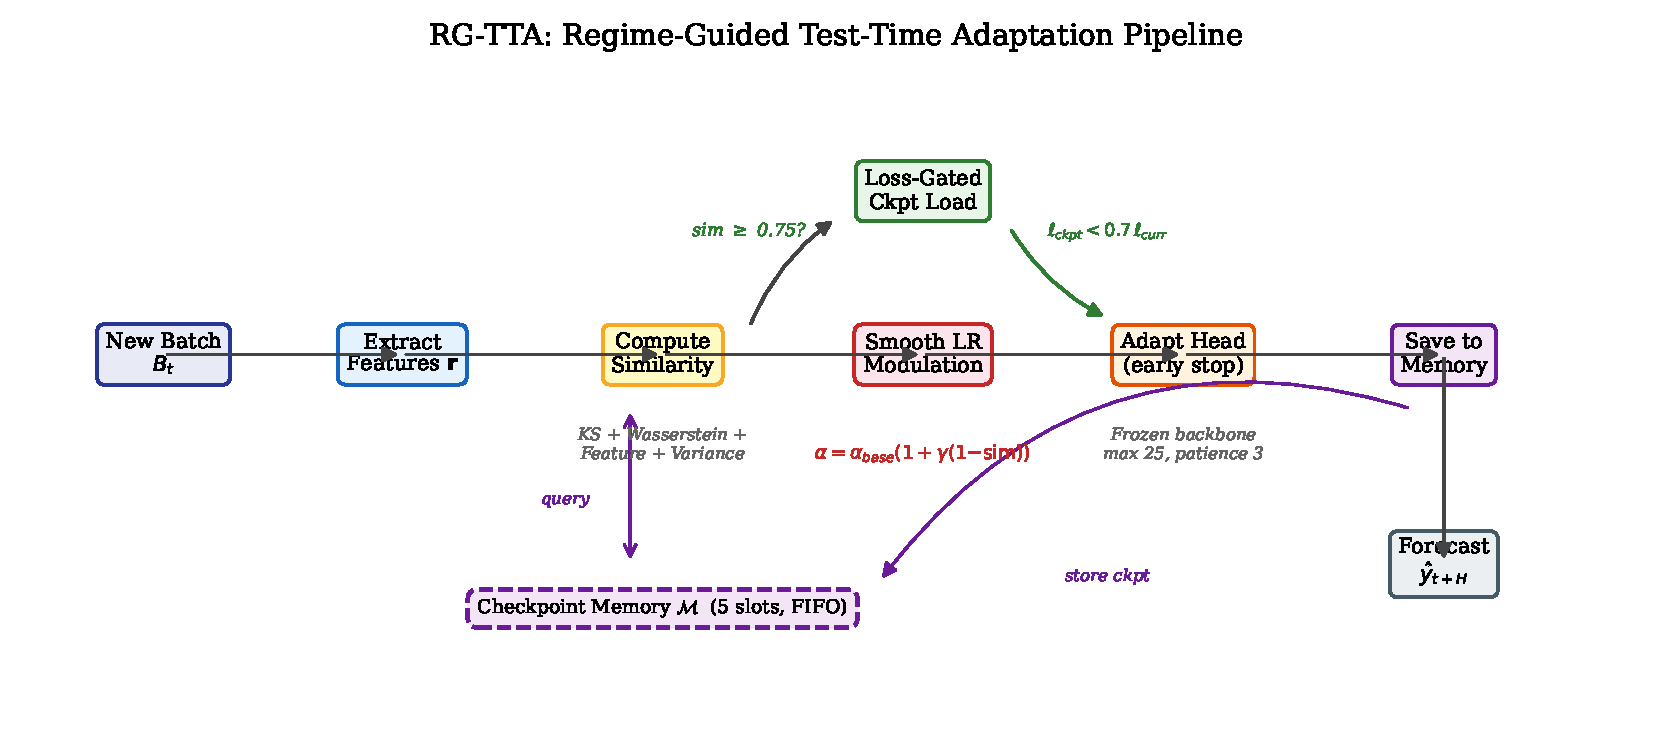
\includegraphics[width=0.95\textwidth]{figures/workflow.pdf}
\caption{RG-TTA system overview. For each incoming batch, the system extracts a distributional feature vector (Eq.~\ref{eq:features}), computes similarity via a four-metric ensemble (Eq.~\ref{eq:ensemble}), optionally loads a loss-gated checkpoint, modulates the learning rate by similarity (Eq.~\ref{eq:lr}), and adapts with early stopping. The adapted checkpoint is stored for future reuse.}
\label{fig:workflow}
\end{figure*}

\subsection{Problem Setup}

Data arrives as a stream of batches $B_1, B_2, \ldots$ (batch size 750). A base forecaster $f_\theta$ can be trained, saved, and loaded. At each step $t$, the system produces a forecast $\hat{y}_{t+1:t+H}$ for horizon $H \in \{96, 192, 336, 720\}$ and optionally updates $\theta$. All 6 policies share the same architecture, data splits, and seeds; only the update rule differs.

\subsection{Distributional Similarity Metric}
\label{sec:similarity}

For each batch, RG-TTA extracts a 5-dimensional distributional feature vector:
\begin{equation}
  \mathbf{r} = \big(\mu,\; \sigma,\; \gamma_1,\; \kappa{-}3,\; r_1\big),
  \label{eq:features}
\end{equation}
where $\mu$ is the mean, $\sigma$ the standard deviation, $\gamma_1$ the skewness, $\kappa{-}3$ the excess kurtosis, and $r_1$ the lag-1 autocorrelation. These features capture the distribution's location, scale, shape, tail behaviour, and temporal structure in $O(n)$ time.

Similarity between a query batch $\mathbf{q}$ and a stored regime $\mathbf{s}$ uses a weighted ensemble of four metrics:

\paragraph{Kolmogorov--Smirnov similarity.} $\text{sim}_{\text{KS}} = 1 - D_n$, where $D_n = \sup_x |F_{\mathbf{q}}(x) - F_{\mathbf{s}}(x)|$ is the two-sample KS statistic~\cite{massey1951ks}.

\paragraph{Wasserstein-1 similarity.} $\text{sim}_{\text{W}} = (1 + W_1 / \max(\text{ptp}(\mathbf{q}), \text{ptp}(\mathbf{s}), \epsilon))^{-1}$, the normalised earth-mover's distance~\cite{villani2009optimal}.

\paragraph{Feature-distance similarity.} $\text{sim}_{\text{feat}} = (1 + \|\mathbf{q} - \mathbf{s}\|_2 / ((\|\mathbf{q}\|_2 + \|\mathbf{s}\|_2)/2 + \epsilon))^{-1}$.

\paragraph{Variance-ratio similarity.} $\text{sim}_{\text{var}} = \min(\sigma_{\mathbf{q}}, \sigma_{\mathbf{s}}) / (\max(\sigma_{\mathbf{q}}, \sigma_{\mathbf{s}}) + \epsilon)$.

\paragraph{Weighted ensemble.}
\begin{equation}
  \text{sim}(\mathbf{q}, \mathbf{s}) = 0.3 \cdot \text{sim}_{\text{KS}} + 0.3 \cdot \text{sim}_{\text{W}} + 0.2 \cdot \text{sim}_{\text{feat}} + 0.2 \cdot \text{sim}_{\text{var}}.
  \label{eq:ensemble}
\end{equation}
The statistical tests (KS, Wasserstein) receive higher weight as they are non-parametric and capture arbitrary shape differences. Ablation confirms the ensemble outperforms every single-metric variant (Table~\ref{tab:ablation_main}; detailed analysis in Supplementary~\S{S5}).

\subsection{Continuous Regime-Guided Adaptation}
\label{sec:adaptation}

RG-TTA uses the similarity score as a \emph{continuous} control signal:

\paragraph{Smooth learning rate modulation.}
\begin{equation}
  \alpha = \alpha_{\text{base}} \cdot \big(1 + \gamma \cdot (1 - \text{sim})\big),
  \label{eq:lr}
\end{equation}
where $\alpha_{\text{base}} = 3 \times 10^{-4}$ and $\gamma = 0.67$. At $\text{sim} = 1.0$, $\alpha = \alpha_{\text{base}}$ (conservative); at $\text{sim} = 0.0$, $\alpha \approx 1.67 \times \alpha_{\text{base}}$ (aggressive).

\paragraph{Loss-gated checkpoint reuse.} When the best-matching regime has $\text{sim} \geq 0.75$, RG-TTA evaluates the stored checkpoint via a forward pass. The checkpoint is loaded only if:
\begin{equation}
  \ell_{\text{ckpt}} < 0.70 \cdot \ell_{\text{curr}},
  \label{eq:gate}
\end{equation}
requiring $\geq$30\% loss improvement over the current model.

\paragraph{Loss-driven early stopping.} RG-TTA runs up to $K_{\max} = 25$ steps with early stopping: if relative improvement falls below $\epsilon = 0.005$ for 3 consecutive steps (after $K_{\min} = 5$), adaptation halts. In practice, RG-TTA averages 18.5 steps per batch vs TTA's fixed 20.

Algorithm~\ref{alg:rgtta} gives the pseudocode.

\begin{algorithm}[t]
\caption{RG-TTA: Regime-Guided Test-Time Adaptation}
\label{alg:rgtta}
\begin{algorithmic}[1]
\REQUIRE Batch $B_t$, checkpoint memory $\mathcal{M}$, base LR $\alpha_{\text{base}}$, scale $\gamma$, gate $g$
\STATE $\mathbf{q} \leftarrow \text{features}(B_t)$ \hfill \COMMENT{Eq.~\ref{eq:features}}
\STATE $(\text{sim}^*, \theta^*_{\text{ckpt}}) \leftarrow \max_{\mathbf{s} \in \mathcal{M}} \text{sim}(\mathbf{q}, \mathbf{s})$ \hfill \COMMENT{Eq.~\ref{eq:ensemble}}
\STATE $\ell_{\text{curr}} \leftarrow \mathcal{L}(f_\theta(X_t), y_t)$
\IF{$\text{sim}^* \geq 0.75$}
  \STATE $\ell_{\text{ckpt}} \leftarrow \mathcal{L}(f_{\theta^*_{\text{ckpt}}}(X_t), y_t)$
  \IF{$\ell_{\text{ckpt}} < g \cdot \ell_{\text{curr}}$}
    \STATE $\theta \leftarrow \theta^*_{\text{ckpt}}$; \, $\ell_{\text{curr}} \leftarrow \ell_{\text{ckpt}}$
  \ENDIF
\ENDIF
\STATE $\alpha \leftarrow \alpha_{\text{base}} \cdot (1 + \gamma \cdot (1 - \text{sim}^*))$ \hfill \COMMENT{Eq.~\ref{eq:lr}}
\STATE patience $\leftarrow 0$
\FOR{$k = 1$ to $K_{\max}$}
  \STATE $\hat{y} = f_{\theta_{\text{head}}}(X_t)$ \hfill \COMMENT{Backbone frozen}
  \STATE $\mathcal{L} = \text{SmoothL1}(\hat{y}, y_t)$~\cite{huber1964robust} \hfill \COMMENT{+ optional EWC/DynaTTA}
  \STATE $\theta_{\text{head}} \leftarrow \theta_{\text{head}} - \alpha \nabla_{\theta_{\text{head}}} \mathcal{L}$
  \IF{$k \geq K_{\min}$ \AND $(\ell_{k-1} - \ell_k)/|\ell_{k-1}| < \epsilon$}
    \STATE patience $\leftarrow$ patience $+ 1$
    \IF{patience $\geq 3$} \STATE \textbf{break} \ENDIF
  \ELSE
    \STATE patience $\leftarrow 0$
  \ENDIF
\ENDFOR
\STATE $\mathcal{M}[\mathbf{q}] \leftarrow (\theta, \text{metadata})$ \hfill \COMMENT{Store for future reuse}
\RETURN $\hat{y}_{t+1:t+H}$
\end{algorithmic}
\end{algorithm}

\subsection{RG-EWC and RG-DynaTTA Variants}
\label{sec:variants}

\paragraph{RG-EWC.} Adds EWC regularisation~\cite{kirkpatrick2017ewc} to RG-TTA:
\begin{equation}
  \mathcal{L}_{\text{total}} = \mathcal{L}_{\text{task}} + \frac{\lambda}{2} \sum_i F_i (\theta_i - \theta^*_i)^2,
  \label{eq:ewc}
\end{equation}
where $F_i$ is the diagonal Fisher Information ($\lambda = 400$, 200 samples, online EMA decay 0.5). When a checkpoint is loaded, the EWC anchor resets to prevent penalising movement away from the pre-load state. RG-EWC reduces MSE by 14.1\% vs standalone EWC (75.4\% win rate).

\paragraph{RG-DynaTTA.} Combines proactive regime detection with reactive shift-magnitude sensing~\cite{grover2025dynatta}. DynaTTA's sigmoid formula computes the LR based on prediction-error z-scores and embedding distances, creating a two-level controller: RG-TTA provides checkpoint reuse and early stopping; DynaTTA provides continuous LR within $[\alpha_{\min}, \alpha_{\max}]$.

\subsection{Checkpoint Management and Frozen Backbone}
\label{sec:checkpoints}

Each checkpoint stores model weights, the 5-D feature vector, raw batch values, and the fitted preprocessor state. The memory is capped at 5 entries with FIFO eviction.

All gradient-based policies freeze the backbone during adaptation and update only the output projection layer ($\sim$5--50\% of parameters, depending on architecture). This mirrors linear probing in vision TTA and provides implicit regularisation. The effectiveness is architecture-dependent: strongest for recurrent/linear models, weaker for attention-based architectures where attention patterns also need shifting (Supplementary~\S{S2}).


% ============================================================
\section{Theoretical Analysis}
\label{sec:theory}
% ============================================================

We provide formal analysis of RG-TTA's design pillars. The analysis assumes strong convexity and smoothness of the output-head loss---reasonable for the single linear layer that constitutes the trainable head, but an idealisation relative to Adam and finite-batch noise. The results should be read as \emph{design rationale and directional guarantees}; the empirical results in \S\ref{sec:results} provide the definitive evaluation. Full proofs are in Supplementary~\S{S3}.

\subsection{Adaptation Error Decomposition}

Let $f_\theta = h_\phi \circ g_\psi$ where $g_\psi$ is the frozen backbone and $h_\phi$ is the trainable output head. Let $\phi^*_t = \arg\min_\phi \mathbb{E}_{P_t}[\ell(h_\phi(g_\psi(x)), y)]$.

\begin{theorem}[Adaptation error bound]
\label{thm:adaptation}
Assume the per-batch loss is $\mu$-strongly convex and $L$-smooth in $\phi$ with $\kappa = L/\mu$. After $K$ gradient descent steps with $\alpha \in (0, 2/L)$ from $\phi_0$:
\begin{equation}
    \|\phi_K - \phi^*_t\|^2 \leq \rho^{2K} \|\phi_0 - \phi^*_t\|^2, \quad \rho = 1 - \frac{2\mu\alpha}{1 + \mu\alpha} < 1.
    \label{eq:gd_rate}
\end{equation}
The expected per-batch MSE decomposes as:
\begin{equation}
    \mathbb{E}[\ell(\phi_K)] = \underbrace{\sigma^2_t}_{\textup{irreducible}} + \underbrace{\rho^{2K} \|\phi_0 - \phi^*_t\|^2_H}_{\textup{adaptation residual}}.
    \label{eq:error_decomp}
\end{equation}
\end{theorem}

When RG-TTA loads a checkpoint with similarity $s$, the initialisation error satisfies $\|\phi_{\textup{ckpt}} - \phi^*_t\|^2 \leq (1-s)^2 D^2_{\max}$, yielding:
\begin{equation}
    \mathbb{E}[\ell^{\textup{RG}}(\phi_K)] \leq \sigma^2_t + \rho^{2K}(1-s)^2 D^2_{\max}.
    \label{eq:rg_error}
\end{equation}
This reveals three mechanisms for reducing error: more steps $K$ (TTA), better initialisation via $(1{-}s)^2$ (RG-TTA), or both.

\begin{corollary}[Step savings]
\label{cor:steps}
The per-batch step savings from checkpoint loading are $\Delta K = -\log(1{-}s)/|\log\rho|$. For $s = 0.85$ and $\rho = 0.95$: $\Delta K \approx 37$ steps---exceeding $K_{\max}$, meaning the checkpoint is near-optimal and early stopping activates within $K_{\min}$ steps.
\end{corollary}

\subsection{Generalisation Bound under Frozen Backbone}

\begin{theorem}[Generalisation bound]
\label{thm:generalization}
Let $\mathcal{F}_{\textup{frozen}} = \{x \mapsto h_\phi(g_{\psi^*}(x)) : \phi \in \Phi\}$ with linear head $h_\phi(z) = Wz + b$, $\|W\|_F \leq B_W$, $\|g_{\psi^*}(x)\| \leq C_g$. For $n$ i.i.d.\ samples with bounded loss $\ell \in [0, c]$, with probability $\geq 1-\delta$:
\begin{equation}
    R(\hat{f}) \leq \hat{R}_n(\hat{f}) + \frac{2 c_\ell B_W C_g}{\sqrt{n}} + 3\sqrt{\frac{\ln(2/\delta)}{2n}}.
    \label{eq:gen_bound}
\end{equation}
The complexity ratio $\hat{\mathfrak{R}}_n(\mathcal{F}_{\textup{frozen}}) / \hat{\mathfrak{R}}_n(\mathcal{F}_{\textup{full}}) \propto \sqrt{d_{\textup{head}}/d_{\textup{total}}} \approx 0.38$ for GRU-Small---a ${\sim}2.6\times$ tighter bound than full-model adaptation.
\end{theorem}

\subsection{Metric Properties and Checkpoint Loading}

\begin{proposition}[Metric properties]
\label{prop:metric}
The ensemble similarity (Eq.~\ref{eq:ensemble}) satisfies: (1)~boundedness in $[0,1]$, (2)~self-similarity, (3)~symmetry, (4)~statistical consistency, and (5)~discriminative power ($\textup{sim}(P,Q) = 1 \Rightarrow P = Q$ for continuous distributions).
\end{proposition}

\begin{proposition}[Checkpoint loading condition]
\label{prop:loading}
Under $\mu$-strong convexity, the loss gate $\ell(\phi_{\textup{ckpt}}) < 0.70 \cdot \ell(\phi_{\textup{curr}})$ implies $\|\phi_{\textup{ckpt}} - \phi^*_t\| \leq 0.84\|\phi_{\textup{curr}} - \phi^*_t\|$, guaranteeing beneficial loading.
\end{proposition}


% ============================================================
\section{Experiments}
\label{sec:experiments}
% ============================================================

\subsection{Setup}

We evaluate on 14 datasets: 6 real-world benchmarks (ETTh1, ETTh2, ETTm1, ETTm2~\cite{zhou2021informer}, Weather~\cite{wu2021autoformer}, Exchange~\cite{lai2018modeling}) and 8 synthetic regime scenarios isolating specific adaptation challenges (stable, trend break, slow drift, fast switch, recurring, volatility, shock recovery, multi-regime). Dataset details are in Supplementary~\S{S6}.

Four compact architectures (37K--192K parameters) span recurrent (GRU~\cite{cho2014gru}, $\sim$71K), attention (iTransformer~\cite{liu2024itransformer}, $\sim$123K; PatchTST~\cite{nie2023patchtst}, $\sim$192K), and linear (DLinear~\cite{zeng2023dlinear}, $\sim$37K) families. All policies use the same model per experiment.

Six policies form a controlled hierarchy (Table~\ref{tab:policies}): each RG-variant differs from its baseline only in adding the regime-guidance layer, isolating the contribution of regime-awareness.

\begin{table}[t]
\centering
\caption{The 6 update policies. Policies 1--3 are baselines; 4--6 are our contributions.}
\label{tab:policies}
\small
\resizebox{\columnwidth}{!}{%
\begin{tabular}{clcccl}
\toprule
\# & Policy & Steps & LR & Mem. & Key mechanism \\
\midrule
1 & TTA & 20 & $3{\times}10^{-4}$ & No & Fixed-step gradient \\
2 & EWC & 15 & $3{\times}10^{-4}$ & No & Fisher-penalised \\
3 & DynaTTA & 20 & Dynamic & No & Sigmoid LR \\
\midrule
4 & \textbf{RG-TTA} & $\leq$25 & Sim-scaled & Yes & Regime-guided TTA \\
5 & \textbf{RG-EWC} & $\leq$25 & Sim-scaled & Yes & + EWC ($\lambda$=400) \\
6 & \textbf{RG-DynaTTA} & $\leq$25 & DynaTTA+RG & Yes & + DynaTTA LR \\
\bottomrule
\end{tabular}
}% end resizebox
\end{table}

\paragraph{Evaluation protocol.} Streaming: initial training on 720 rows, then sequential processing of up to 10 batches of 750 rows each. This reflects production deployment (batch-wise updates) and preserves RG-TTA's full decision space (how many steps, at what LR, from which starting point). Full protocol justification is in Supplementary~\S{S7}.

\paragraph{Metrics.} MSE (primary), MAE, RMSE, sMAPE, wMAPE, direction accuracy. Statistical significance via Wilcoxon signed-rank tests~\cite{wilcoxon1945} with Bonferroni correction; overall ranking via Friedman test~\cite{friedman1937} with Nemenyi post-hoc~\cite{demsar2006statistical}.


% ============================================================
\section{Results}
\label{sec:results}
% ============================================================

We present results from 672 experiments (6 policies $\times$ 4 models $\times$ 14 datasets $\times$ 4 horizons $\times$ 3 seeds). All tables report seed-averaged values (224 unique experiments).

\subsection{Overall Win Counts}

\begin{table}[t]
\centering
\caption{Win counts across 224 seed-averaged experiments. Regime-guided policies (ours) win 156/224 (69.6\%).}
\label{tab:wins}
\small
\begin{tabular}{lcc}
\toprule
Policy & Wins & Win Rate \\
\midrule
TTA & 46 & 20.5\% \\
EWC & 13 & 5.8\% \\
DynaTTA & 9 & 4.0\% \\
\midrule
\textbf{RG-TTA} & \textbf{65} & \textbf{29.0\%} \\
\textbf{RG-EWC} & \textbf{68} & \textbf{30.4\%} \\
\textbf{RG-DynaTTA} & 23 & 10.3\% \\
\midrule
\emph{Our total} & \emph{156} & \emph{69.6\%} \\
\bottomrule
\end{tabular}
\end{table}

Table~\ref{tab:wins} shows that regime-guided policies win 69.6\% of experiments, with RG-EWC (30.4\%) and RG-TTA (29.0\%) nearly tied as the strongest individual policies. Notably, the win rates on real-world (69.8\%) and synthetic (69.5\%) datasets are near-identical, ruling out inflation from synthetic data design.

\subsection{Pair-wise Regime-Guidance Effect}

\begin{table*}[t]
\centering
\caption{Head-to-head: each baseline vs its regime-guided variant. $\Delta$MSE is average relative change (negative = RG-variant better). $p$-values from one-sided Wilcoxon signed-rank tests with Bonferroni correction ($\alpha = 0.05/3$).}
\label{tab:pairwise}
\small
\begin{tabular}{llcccc}
\toprule
Baseline & RG-Variant & $\Delta$MSE (avg) & $\Delta$MSE (med.) & RG Wins & $p$-value \\
\midrule
TTA & RG-TTA & $-5.7\%$ & $-5.1\%$ & 150/224 (67.0\%) & $1.0{\times}10^{-5}$\rlap{***} \\
EWC & RG-EWC & $-14.1\%$ & $-10.0\%$ & 169/224 (75.4\%) & $2.4{\times}10^{-11}$\rlap{***} \\
DynaTTA & RG-DynaTTA & $+0.5\%$ & $-3.8\%$ & 139/224 (62.1\%) & $6.8{\times}10^{-3}$\rlap{**} \\
\bottomrule
\end{tabular}
\vspace{2pt}
\par\footnotesize ***$p<0.001$, **$p<0.01$. All three pairs significant after Bonferroni correction.
\end{table*}

Table~\ref{tab:pairwise} isolates the regime-guidance effect. RG-EWC shows the strongest benefit ($-14.1\%$ MSE, 75.4\% win rate). All three improvements are statistically significant (Wilcoxon, $p < 0.007$, Bonferroni-corrected). The composability claim holds empirically: regime-guidance improves all three base methods. Figure~\ref{fig:pairwise} visualises the pair-wise effects.

\begin{figure}[t]
\centering
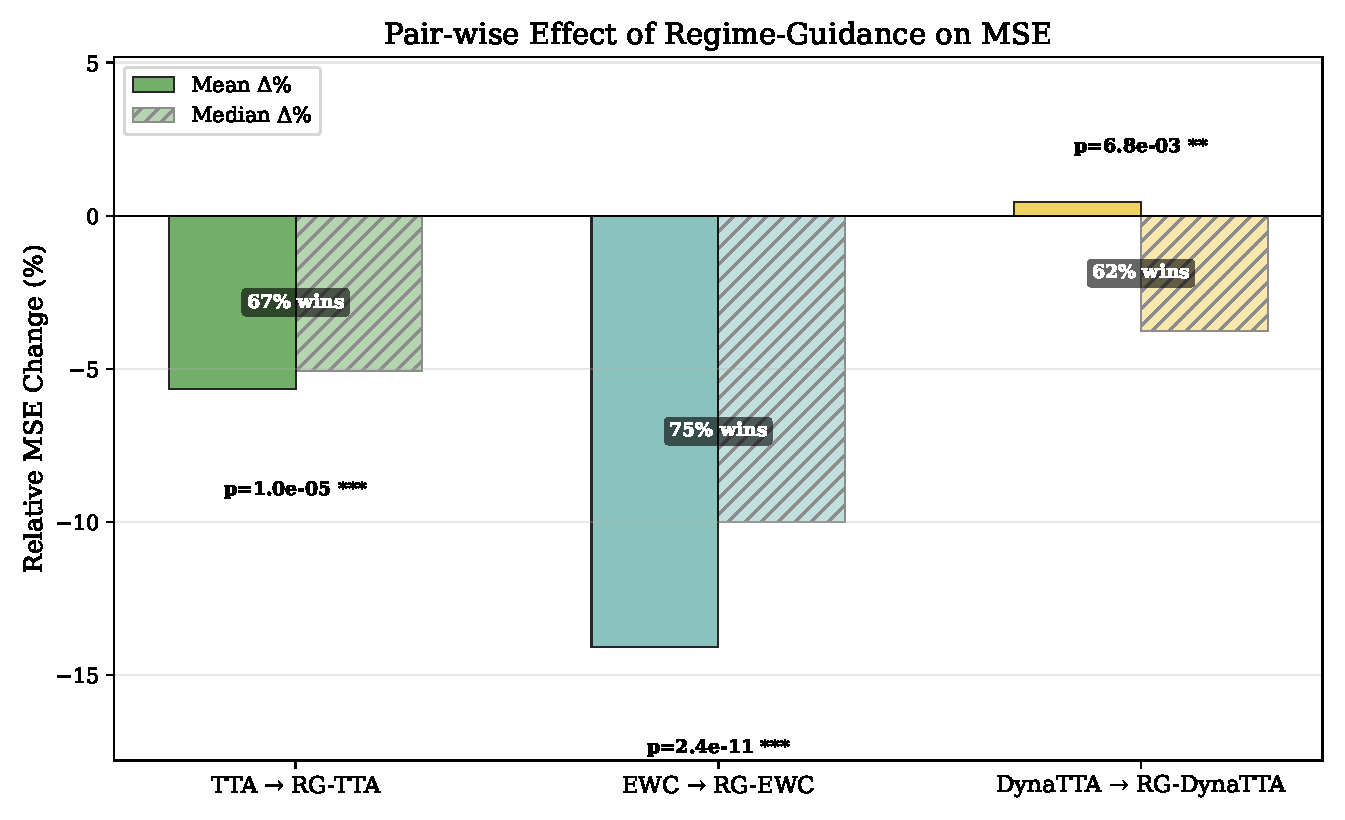
\includegraphics[width=\columnwidth]{figures/pairwise_improvement.pdf}
\caption{Pair-wise MSE change from adding regime-guidance. Negative = improvement. All pairs statistically significant.}
\label{fig:pairwise}
\end{figure}

\subsection{MSE by Model Architecture}

\begin{table}[t]
\centering
\caption{Average MSE across 14 datasets $\times$ 4 horizons, by policy and model. \textbf{Bold} = best per column. Synthetic datasets dominate due to scale; see Table~\ref{tab:realworld} for real-world results.}
\label{tab:main}
\small
\resizebox{\columnwidth}{!}{%
\begin{tabular}{lrrrr}
\toprule
Policy & GRU-S & iTransformer & PatchTST & DLinear \\
\midrule
TTA & 15,458 & 21,075 & 717,298 & 17,855 \\
EWC & 16,794 & 24,141 & 813,314 & 18,258 \\
DynaTTA & 16,076 & 20,808 & 874,257 & 17,185 \\
\midrule
\textbf{RG-TTA} & \textbf{14,092} & 19,202 & \textbf{718,642} & 18,782 \\
\textbf{RG-EWC} & \textbf{14,047} & \textbf{18,851} & 721,305 & 18,752 \\
\textbf{RG-DynaTTA} & 16,787 & 22,619 & 868,742 & \textbf{16,739} \\
\bottomrule
\end{tabular}
}% end resizebox
\end{table}

RG-TTA and RG-EWC are best on GRU-Small ($-8.8\%$ and $-9.1\%$ vs TTA) and iTransformer ($-8.9\%$ and $-10.6\%$). On PatchTST, policies cluster tightly (TTA edges RG-TTA by $<0.2\%$). On DLinear, RG-DynaTTA wins ($-2.6\%$ vs DynaTTA). The advantage is strongest on recurrent models where the frozen backbone preserves reusable temporal features.

\subsection{Statistical Ranking}

The Friedman test~\cite{friedman1937} across 224 experiments overwhelmingly rejects the null ($\chi^2 = 301.95$, $p = 3.81 \times 10^{-63}$). Average ranks (lower is better): RG-TTA 2.46, RG-EWC 2.51, TTA 2.98, EWC 4.02, RG-DynaTTA 4.34, DynaTTA 4.69. The Nemenyi post-hoc test (CD $= 0.50$, $\alpha = 0.05$) confirms RG-TTA and RG-EWC are statistically indistinguishable and both significantly better than all other policies (Fig.~\ref{fig:cd}).

\begin{figure}[t]
\centering
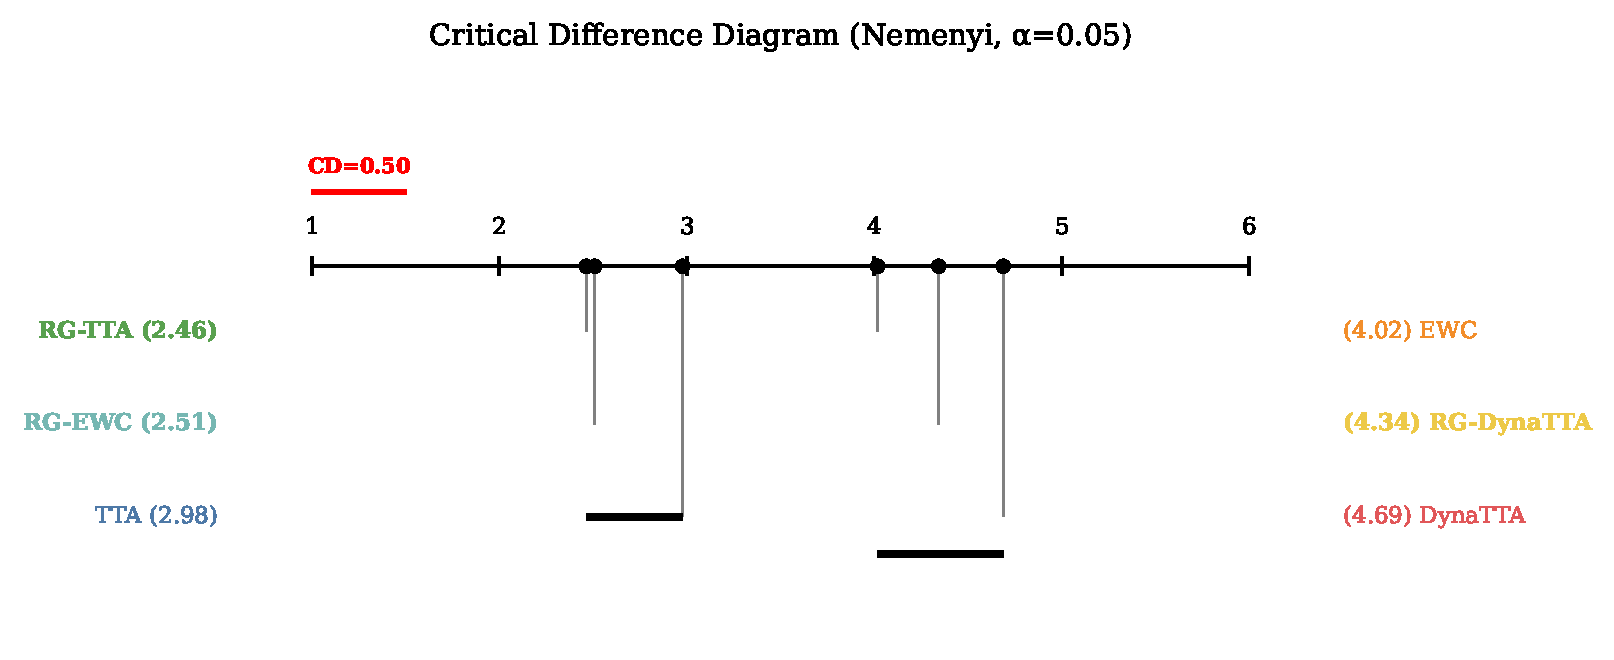
\includegraphics[width=\columnwidth]{figures/critical_difference.pdf}
\caption{Critical difference diagram (Nemenyi, $\alpha=0.05$). Connected policies are not significantly different. RG-TTA and RG-EWC rank best.}
\label{fig:cd}
\end{figure}

\subsection{Real-World Benchmark Results}

\begin{table*}[t]
\centering
\caption{Average MSE on real-world datasets (4 horizons $\times$ 4 models $\times$ 3 seeds). \textbf{Bold} = best per column.}
\label{tab:realworld}
\small
\begin{tabular}{lrrrrrr}
\toprule
Policy & ETTh1 & ETTh2 & ETTm1 & ETTm2 & Weather & Exchange \\
\midrule
TTA & 56.15 & 92.54 & 20.88 & 40.53 & \textbf{138.99} & 0.01 \\
EWC & 63.80 & 102.21 & 23.40 & 42.89 & 147.67 & 0.01 \\
DynaTTA & 89.29 & 130.18 & 24.62 & 45.49 & 164.37 & 0.01 \\
\midrule
\textbf{RG-TTA} & 53.74 & 78.99 & \textbf{18.05} & 37.69 & 145.21 & \textbf{0.01} \\
\textbf{RG-EWC} & \textbf{52.33} & \textbf{78.41} & 18.14 & \textbf{37.10} & 151.39 & \textbf{0.01} \\
\textbf{RG-DynaTTA} & 79.90 & 127.21 & 25.22 & 41.79 & 175.31 & 0.01 \\
\bottomrule
\end{tabular}
\end{table*}

RG-TTA and RG-EWC achieve the best MSE on 5 of 6 real-world datasets (Table~\ref{tab:realworld}). The exception is \textbf{Weather}, where TTA wins---its 21-feature structure and gradual drift favour fixed-step adaptation over similarity-modulated updates. On \textbf{Exchange}, all policies perform identically, confirming regime-guidance neither helps nor hurts on random-walk data.

\subsection{Dataset Category Analysis}

\begin{table}[t]
\centering
\caption{Average MSE by dataset category and policy, averaged across models and horizons.}
\label{tab:bycategory}
\small
\resizebox{\columnwidth}{!}{%
\begin{tabular}{lrrrr}
\toprule
Policy & ETT (4) & Weather+Exch. (2) & Synth-Recur. (3) & Synth-Shock (5) \\
\midrule
TTA & 52.53 & 69.50 & 292,818 & 364,420 \\
EWC & 58.08 & 73.84 & 338,101 & 407,818 \\
DynaTTA & 72.40 & 82.19 & 366,484 & 429,847 \\
\midrule
\textbf{RG-TTA} & \textbf{47.12} & 72.61 & 300,952 & \textbf{358,865} \\
\textbf{RG-EWC} & \textbf{46.50} & 75.70 & 303,245 & 359,054 \\
\textbf{RG-DynaTTA} & 68.53 & 87.66 & 357,825 & 432,636 \\
\bottomrule
\end{tabular}
}% end resizebox
\end{table}

RG-TTA and RG-EWC dominate on ETT datasets ($-10.3\%$ and $-11.5\%$ vs TTA). While these datasets exhibit recurring patterns in electricity consumption, checkpoint loading fires on only 2--7\% of batches (\S\ref{sec:ablation}). The gains are primarily driven by the similarity-modulated LR and loss-driven early stopping.

\subsection{Per-Dataset Win Rates}

Of the 14 datasets, regime-guided policies win the majority on 13. Notable win rates: synth\_recurring (\textbf{100\%}), ETTh2 (88\%), synth\_trend\_break (88\%), ETTh1 (81\%), synth\_shock\_recovery (81\%). The only weak datasets are Weather (38\%) and synth\_volatility (6\%). The 100\% win rate on \texttt{synth\_recurring} comes entirely from the similarity-modulated LR---checkpoint loading never fires because the live model already adapts well. Full per-dataset breakdown in Supplementary~\S{S4.3}.

\subsection{Computational Cost}

\begin{table}[t]
\centering
\caption{Average total adaptation time (seconds) per experiment. Lower is better.}
\label{tab:time}
\small
\resizebox{\columnwidth}{!}{%
\begin{tabular}{lrrrrr}
\toprule
Policy & GRU-S & iTransf. & PatchTST & DLinear & Overall \\
\midrule
TTA & 106.3 & 33.5 & 381.1 & 16.1 & 134.3 \\
EWC & 253.2 & 42.3 & 312.8 & 17.0 & 156.4 \\
DynaTTA & 121.9 & 34.7 & 411.8 & 17.2 & 146.4 \\
\midrule
\textbf{RG-TTA} & 118.7 & 38.7 & 335.7 & 14.5 & \textbf{126.9} \\
\textbf{RG-EWC} & 286.7 & 55.0 & 360.2 & 19.1 & 180.3 \\
\textbf{RG-DynaTTA} & 129.0 & 36.9 & 421.2 & 17.0 & 151.0 \\
\bottomrule
\end{tabular}
}% end resizebox
\end{table}

RG-TTA is \emph{faster} than all baselines (126.9s vs TTA's 134.3s, $-5.5\%$), thanks to early stopping on familiar batches. RG-EWC is 15.3\% slower than EWC but gains 14.1\% in MSE. The regime-detection overhead ($<$1s per batch) is negligible. Figure~\ref{fig:tradeoff} visualises the MSE--time trade-off.

\begin{figure*}[t]
\centering
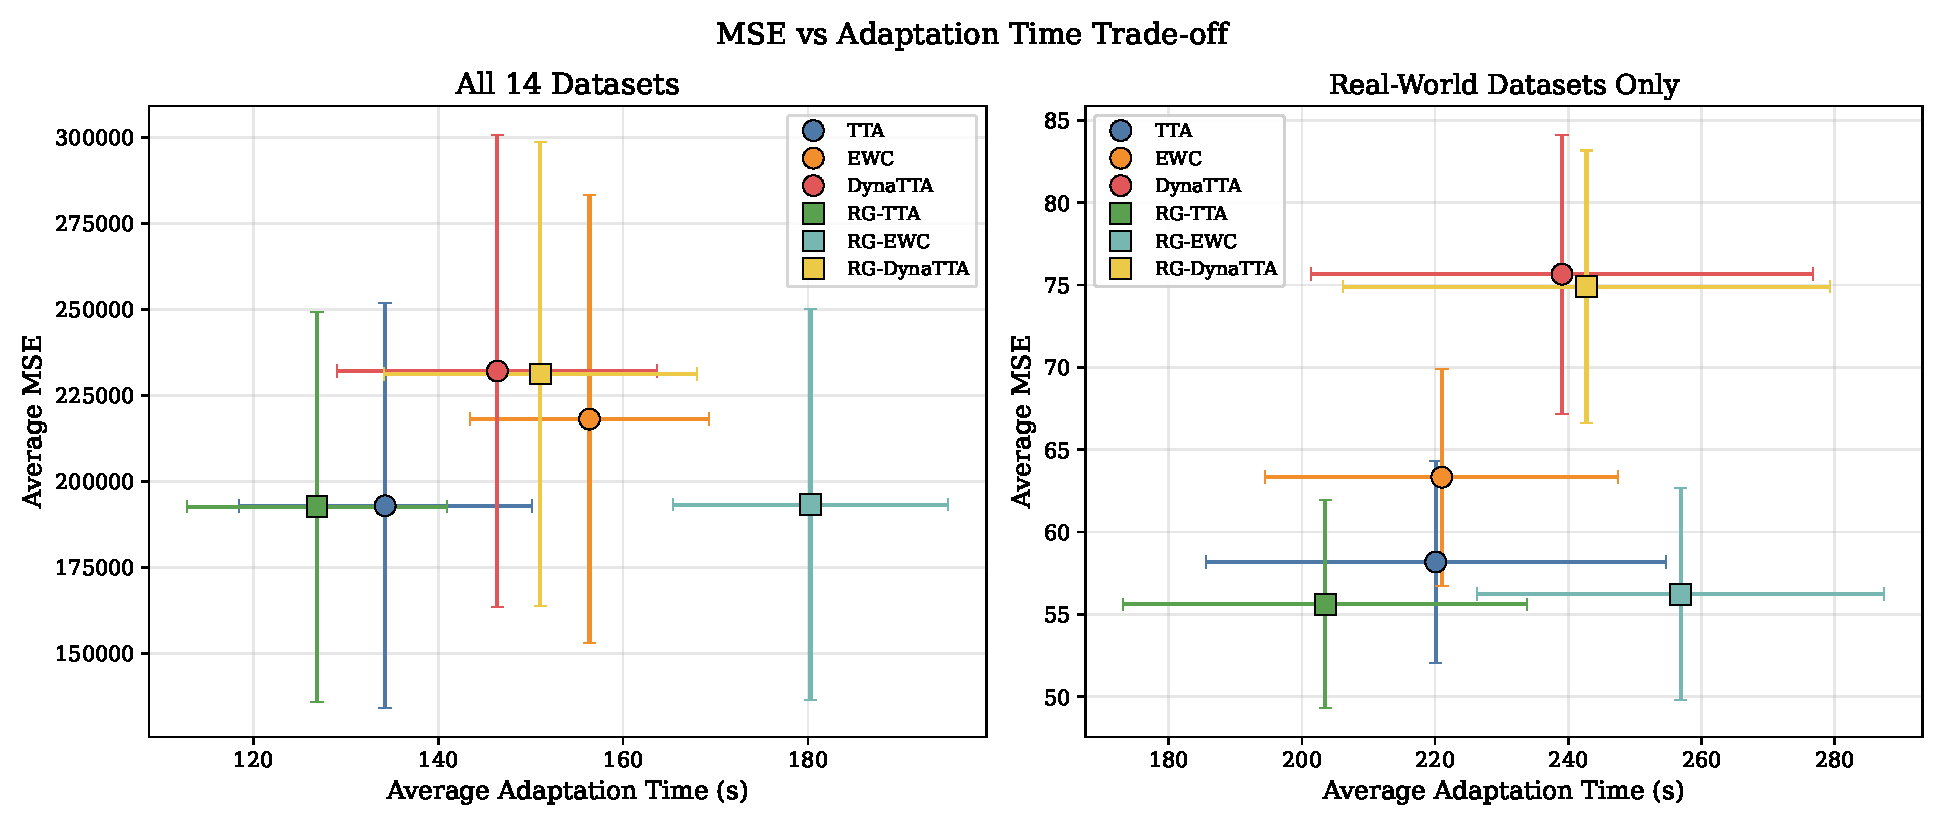
\includegraphics[width=0.95\textwidth]{figures/mse_vs_time.pdf}
\caption{MSE vs adaptation time. RG-TTA achieves the best trade-off (lower MSE \emph{and} lower time). Square markers = regime-guided policies.}
\label{fig:tradeoff}
\end{figure*}

\subsection{Horizon Scaling}

RG-TTA and RG-EWC maintain their advantage at all horizons (96--720), with the gap slightly widening at H=720 on real-world data (Fig.~\ref{fig:horizon}). Per-horizon MSE values are in Supplementary~\S{S4.5}.

\begin{figure}[t]
\centering
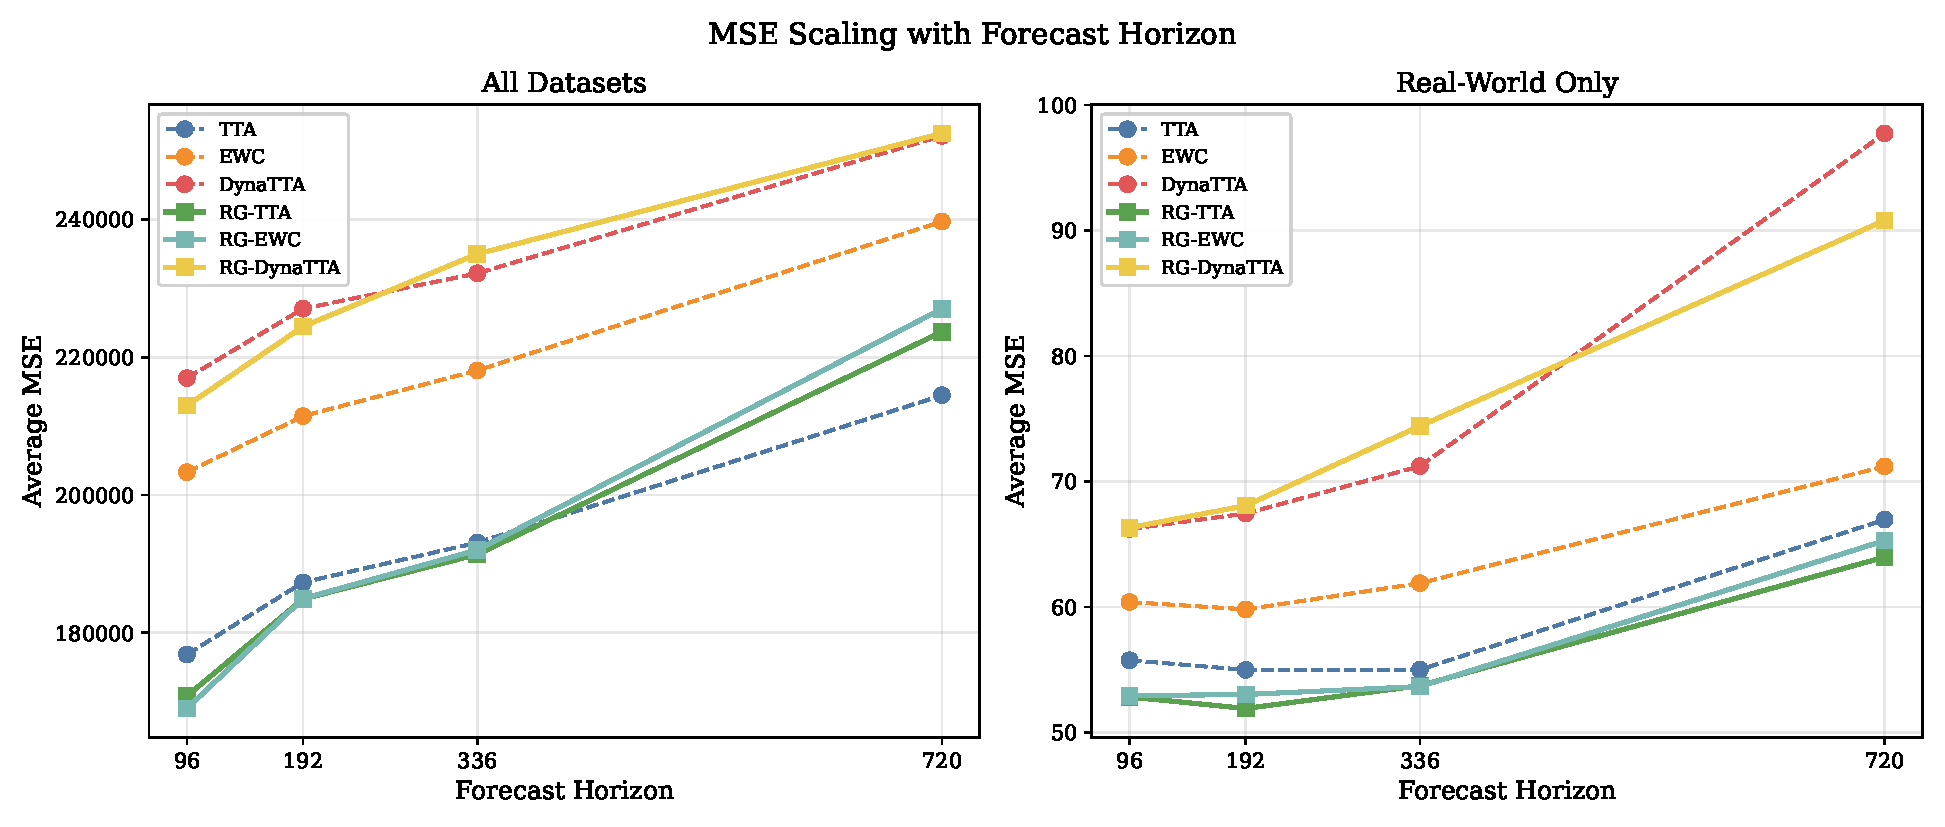
\includegraphics[width=\columnwidth]{figures/horizon_analysis.pdf}
\caption{MSE scaling with forecast horizon. RG-TTA and RG-EWC (solid) outperform baselines (dashed) at all horizons.}
\label{fig:horizon}
\end{figure}

\subsection{Comparison with Full Retraining}
\label{sec:retrain_comparison}

We ran 672 additional retrain experiments (3 architectures; DLinear retrain produced NaN). Regime-guided policies outperform retraining in \textbf{71\%} of 168 configurations (median $-27\%$ MSE). On GRU-Small, RG-EWC achieves $-34\%$ median MSE vs retrain (91\% win rate); on iTransformer, $-40\%$ (84\% win rate). On PatchTST, retrain wins 61\% ($+16\%$ median), benefiting from extended gradient budget. RG-TTA runs 15--30$\times$ faster than retrain. Per-dataset highlights: ETTh2 ($-42\%$, 100\% wins), ETTm1 ($-46\%$, 100\%), Exchange ($-57\%$, 100\%). Retrain's advantage concentrates on synth\_volatility ($+40\%$, 83\% retrain wins).


% ============================================================
\section{Ablation Studies}
\label{sec:ablation}
% ============================================================

We ablate each RG-TTA hyperparameter independently on 4 datasets (ETTh1, ETTm1, synth\_recurring, synth\_shock\_recovery), 2 horizons, 3 seeds (192 experiments). Table~\ref{tab:ablation_main} summarises the results; detailed per-parameter analysis is in Supplementary~\S{S5}.

\begin{table}[t]
\centering
\caption{Hyperparameter sensitivity (MSE averaged over 4 datasets $\times$ 2 horizons $\times$ 3 seeds). Bold = default. TTA baseline = 15{,}515.}
\label{tab:ablation_main}
\small
\resizebox{\columnwidth}{!}{%
\begin{tabular}{llcc}
\toprule
Sweep & Value & MSE & $\Delta$ vs Default \\
\midrule
\multirow{5}{*}{LR scale $\gamma$ (Eq.~\ref{eq:lr})}
  & 0.0 (no modulation) & 16{,}068 & $+17.9\%$ \\
  & 0.33 & 14{,}601 & $+7.2\%$ \\
  & \textbf{0.67} & \textbf{13{,}624} & --- \\
  & 1.0 & 12{,}881 & $-5.5\%$ \\
  & 1.5 & 11{,}966 & $-12.2\%$ \\
\midrule
\multirow{2}{*}{Early stopping}
  & Fixed 20 steps & 15{,}515 & $+13.9\%$ \\
  & \textbf{Loss-driven} & \textbf{13{,}624} & --- \\
\midrule
\multirow{3}{*}{Loss gate $g$}
  & 0.5 & 13{,}624 & $0.0\%$ \\
  & \textbf{0.7} & \textbf{13{,}624} & --- \\
  & 0.9 & 13{,}624 & $0.0\%$ \\
\midrule
\multirow{3}{*}{Memory cap $M$}
  & 1 & 13{,}621 & $0.0\%$ \\
  & \textbf{5} & \textbf{13{,}624} & --- \\
  & 20 & 15{,}442 & $+13.3\%$ \\
\midrule
\multirow{3}{*}{Ckpt threshold $\tau$}
  & 0.65 & 13{,}688 & $+0.5\%$ \\
  & \textbf{0.75} & \textbf{13{,}624} & --- \\
  & 0.85 & 13{,}680 & $+0.4\%$ \\
\midrule
\multirow{2}{*}{Similarity metric}
  & Best single (Wasserstein) & & $+1.8\%$ \\
  & \textbf{Ensemble} & \textbf{---} & --- \\
\bottomrule
\end{tabular}
}% end resizebox
\end{table}

\paragraph{Similarity-modulated LR ($\gamma$).} The most impactful parameter. Its monotonic effect---$\gamma = 0 \rightarrow 0.33 \rightarrow 0.67 \rightarrow 1.0 \rightarrow 1.5$ yields MSE 16{,}068 $\rightarrow$ 14{,}601 $\rightarrow$ 13{,}624 $\rightarrow$ 12{,}881 $\rightarrow$ 11{,}966---provides the strongest evidence that the similarity signal is genuinely informative. Setting $\gamma{=}0$ (no modulation) performs \emph{worse than plain TTA} (16{,}068 vs 15{,}515). The improvement comes from \emph{conditional allocation}: conservative updates on familiar distributions and aggressive updates on novel ones. Our default $\gamma{=}0.67$ is deliberately conservative; higher values further reduce MSE but risk over-adaptation.

\paragraph{Loss-driven early stopping.} Reduces MSE by 13.9\% vs fixed 20 steps while also decreasing wall-clock time by 10\%. The improvement is consistent across all 4 datasets, with the largest gains on datasets with high intra-batch variability (synth\_shock\_recovery: $-14.8\%$).

\paragraph{Robustness.} Four of five hyperparameters show flat optima: loss gate $g$ yields identical MSE across 0.5--0.9 (checkpoint loading is already rare at 2.4\%); memory cap $M \leq 5$ shows $<0.02\%$ variation; checkpoint threshold $\tau$ is stable across 0.70--0.80. Only $M \geq 10$ degrades ($+13.3\%$) due to stale checkpoint interference on recurring synthetic data.

\paragraph{Similarity metric.} The 4-metric ensemble outperforms all single-metric variants (Wasserstein-only: $+1.8\%$, KS-only: $+2.1\%$, variance-ratio-only: $+5.7\%$, feature-only: $+8.3\%$). The ensemble's value lies in complementary coverage: KS detects shape changes, Wasserstein captures location-scale shifts, features capture higher-order moments, and variance ratio captures volatility regimes.

\paragraph{Component contribution.} Across 6{,}672 batch evaluations, checkpoint loading occurs on only 2.4\% of batches (exclusively on real-world datasets: ETTh2 6.9\%, ETTm1/m2 $\sim$7\%; never on synthetic). The primary drivers are the similarity-modulated LR (disabling it degrades MSE by 17.9\%) and loss-driven early stopping. On the 97.6\% of batches without checkpoint loading, RG-TTA still beats TTA on 57.1\% with median $+2.6\%$ improvement. Checkpoint reuse is a valuable supplementary mechanism for datasets with recurring patterns, but not the primary source of overall advantage. Full analysis in Supplementary~\S{S5}.


% ============================================================
\section{Analysis}
\label{sec:analysis}
% ============================================================

\subsection{Computational Complexity}

Per-batch regime-guidance overhead: feature extraction $O(n)$, similarity computation $O(Mn\log n)$ ($M{\leq}5$), checkpoint evaluation $O(M|\theta|)$, memory management $O(M)$. Total: $O(Mn\log n + M|\theta|)$, dominated by gradient steps ($O(K|\theta|)$), adding $<$1s per batch.

\subsection{When RG-TTA Loses}

\paragraph{Continuous drift without recurrence (Weather).} Gradual seasonal drift without regime revisits renders the checkpoint library useless. TTA's fixed 20-step adaptation outperforms by 4.5\%.

\paragraph{Volatility-only shifts (\texttt{synth\_volatility}).} When variance changes but temporal dynamics are unchanged, checkpoints do not help. RG-TTA wins only 6\% of experiments.

\paragraph{Short streams.} RG-TTA needs $\geq$5 batches to build useful memory. On shorter streams, memory is too sparse for effective matching.

\paragraph{Attention architectures with frozen backbone.} Frozen attention layers limit all policies equally on iTransformer and PatchTST.


% ============================================================
\section{Limitations}
\label{sec:limitations}
% ============================================================

\begin{enumerate}[nosep]
  \item \textbf{Compact-model scope.} Designed for $\leq$200K parameters; larger models need more steps than early stopping permits.
  \item \textbf{Conservative LR scaling.} $\gamma{=}1.5$ outperforms default $\gamma{=}0.67$ by 12\%; learned or adaptive $\gamma$ could capture remaining gains.
  \item \textbf{Hand-crafted features.} The 5-D vector is interpretable but may miss complex regime characteristics; learned embeddings could be richer.
  \item \textbf{Univariate regime detection.} Features are computed from the target series only, despite supporting multivariate inputs.
  \item \textbf{Reimplemented baselines.} DynaTTA's codebase is tightly coupled with TAFAS; we reimplemented Algorithm~1 from the published description (details in Supplementary~\S{S1}).
  \item \textbf{DynaTTA protocol mismatch.} DynaTTA's EMA ($\eta{=}0.1$) was designed for 500-window sliding-window evaluation; under our 10-batch protocol, it does not converge (Supplementary~\S{S7}).
  \item \textbf{Architecture-dependent frozen backbone.} Frozen-backbone TTA benefits recurrent/linear models but is less effective for attention architectures.
  \item \textbf{Retrain comparison.} DLinear retrain produced NaN; PatchTST favours retrain (61\% win rate, $+16\%$).
\end{enumerate}


% ============================================================
\section{Conclusion}
\label{sec:conclusion}
% ============================================================

We introduced RG-TTA, a regime-guided meta-controller for test-time adaptation in streaming time series forecasting. RG-TTA continuously modulates adaptation intensity by distributional similarity: familiar distributions get conservative learning rates and early stopping, while novel distributions get aggressive adaptation.

Across 672 experiments, regime-guided policies win 69.6\% of comparisons---with near-identical rates on real-world (69.8\%) and synthetic (69.5\%) data. All pair-wise improvements are statistically significant ($p < 0.007$, Bonferroni-corrected), and the Friedman test rejects equal performance ($p = 3.81 \times 10^{-63}$). Three main findings:

\begin{enumerate}[nosep]
  \item \textbf{RG-EWC is the strongest single policy}, winning 30.4\% and reducing MSE by 14.1\% vs standalone EWC across 75.4\% of comparisons.
  \item \textbf{RG-TTA matches or beats TTA at lower cost}: $-5.7\%$ MSE with $-5.5\%$ wall-clock time.
  \item \textbf{Regime-guidance is composable}: it improves TTA (67\%), EWC (75\%), and DynaTTA (62\%) as a drop-in meta-controller.
\end{enumerate}

Against full retraining, RG policies achieve $-27\%$ median MSE at 15--30$\times$ lower cost (71\% win rate). The practical recommendation is conditional: RG-TTA excels when data streams exhibit recurring distributional regimes; for continuously drifting data, reactive methods suffice.

Code, data, and reproducibility instructions: \repourl.

\IEEEtriggeratref{17}
\bibliographystyle{IEEEtran}
\bibliography{references}

\end{document}
